\documentclass[../main.tex]{subfiles}

\begin{document}


\section{Práctica 2: Creación de un \textit{Board Support Package} (BSP)}

    \subsection{Objetivos}
        \begin{itemize}
            \item Desarrollar un \textit{Board Support Package} minimalista.
            \item Entender la importancia de crear, en la medida de lo posible, código no dependiente del hardware.
        \end{itemize}

    \subsection{Fundamentos teóricos}
       
        Un \textit{Board Support Package} o BSP comprende una colección de bibliotecas que ayudan al programador a trabajar con una placa o procesador determinado. Generalmente, incluyen definiciones, funciones, macros y demás utilidades para que el programador no tenga que trabajar directamente con código de muy bajo nivel como, por ejemplo, hemos hecho en la práctica anterior. Por ejemplo:

        \begin{lstlisting}
            // En lugar de un código así
            * ((uint32_t *) (0x40020000)) &= ~(0b11 << (7*2));
            * ((uint32_t *) (0x40020000)) |=   0b01 << (7*2);

            // Buscamos algo así
            GPIO_SET_MODE(GPIOA, PIN7, MODE_OUTPUT);
        \end{lstlisting}

        Por supuesto, alguien tiene que ser el encargado de crear, por primera vez, este BSP. En sistemas empotrados, normalmente el BSP tiene que ser creado a medida, pues la combinación de procesador, periféricos y pines es particular para cada placa desarrollada. Para la placa \BOARD, ya existe un BSP, y se anima al alumno a consultarlo y ver cómo está construido. A lo largo de estas prácticas, desarrollaremos otro, mucho más minimalista y comedido, que aporte la funcionalidad justa que necesitamos. En esta práctica comenzamos con ese trabajo.

        Vamos a ver el ejemplo concreto de cómo desarrollar la función anterior, para enteder mejor las partes que puede tener un BSP. 

        \subsubsection{Definiciones de direcciones}
            En primer lugar, necesitamos definir las direcciones de memoria donde se encuentran todos nuestros periféricos. Esto cumple una doble función: Por un lado, si cambiaran, las podemos modificar fácilmente al estar definidas como macros. Por otro lado, hacemos el código reutilizable para procesadores de la misma familia (por ejemplo, todos los Cortex-M7 de ARM (como el \MCU que utilizamos) reutilizan partes de los mismos BSPs).

            \begin{lstlisting}
                #define GPIO_BASE_ADDR 0x40020000
                #define GPIOA_BASE_ADDR (GPIO_BASE_ADDR + 0x0000)
                #define GPIOB_BASE_ADDR (GPIO_BASE_ADDR + 0x0400)
                ...
            \end{lstlisting}
        
        \subsubsection{Definiciones de registros}
            Lo siguiente es definir los registros que se encuentran en dichas direcciones. Como suelen ser varios, y consecutivos, se suele definir una estructura de tipo (en lenguaje C) que los englobe todos, por facilidad de uso. Por ejemplo, mirando \REFMAN[6.4.11], podemos ver todos los registros contenidos en cada controlador de GPIO. Se muestra la primera parte de la tabla de registros en la \Cref{fig:gpio_regs}

            \begin{figure}
                \centering
                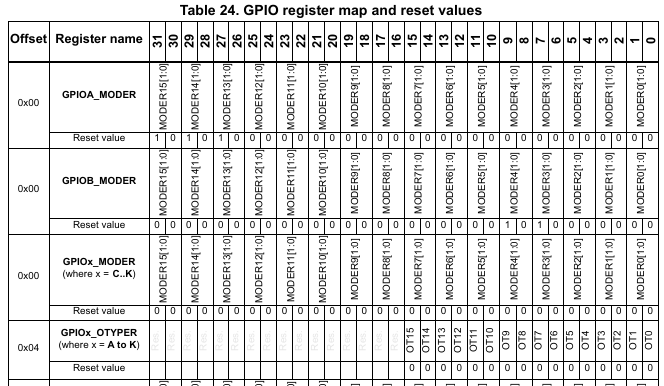
\includegraphics[width=\textwidth]{res/gpio_regs.png}
                \caption{Extracto parcial de registros del controlador de GPIO}
                \label{fig:gpio_regs}
            \end{figure}

            Un detalle interesante a ver aquí es que, por ejemplo, para el registro \REG{MODER}, nos dice que tiene tres valores por defecto (reset) diferentes, según si se trata del puerto A, B, u otros. El registro \REG{TYPER}, sin embargo, tiene el mismo valor por defecto para todos los puertos (A-K). En cada registro, además, nos indica qué bit controla qué cosa. Para los registros \REG{MODER}, los bits, de dos en dos, controlan el modo de GPIO (especificados en \REFMAN[6.4.1]). Para \REG{OTYPER}, controla el tipo de salida (\REFMAN{6.4.2}). Si hacemos el código para tener una estructura que nos permita controlar estos registros, tendríamos algo de este estilo: 

            \begin{lstlisting}
                typedef struct
                {
                    volatile uint32_t MODER;    /*!< GPIO port mode register, Address offset: 0x00      */
                    volatile uint32_t OTYPER;   /*!< GPIO port output type register, Address offset: 0x04      */
                    ...
                } GPIO_TypeDef;
            \end{lstlisting}
            
            Importante observar la declaración de las variables como tipo \lstinline|volatile|, ya que, además de modificarse internamente desde el procesador, son registros cuyo valor puede modificarse desde fuera (por el propio control del periférico). Con la palabra clave \lstinline|volatile| conseguimos que el compilador no optimice esas variables y siempre las consulte directamente de memoria.
            
            \question{¿A qué se debe que todos los registros queden colocados en direcciones sucesivas de memoria al ser declarados con esta sintaxis?}
            \question{Explora qué hace exactamente el compilador al trabajar con objetos volátiles.}

        \subsubsection{Gestión de registros}

            Tenemos definidas las direcciones, y las estructuras de registros. Ahora necesitamos tener una forma de escribir en dichas estructuras. Para ello, vamos a crear punteros a las direcciones de memoria base, con el tipo de estructura definido:

            \begin{lstlisting}
                #define GPIOA               ((GPIO_TypeDef *) GPIOA_BASE_ADDR)
            \end{lstlisting}
            
            Si la base del controlador se encuentra en la dirección \MEMORY{0x40020000} (como es el caso de GPIOA), los registros se encontrarán a continuación (el primero \REG{MODER} en \MEMORY{0x40020000}, el segundo \REG{OTYPER} en \MEMORY{0x40020004}, y así sucesivamente). Así, lo que conseguimos es que, posteriormente, en el código de nuestro programa, podamos hacer algo de este estilo:

            \begin{lstlisting}
                GPIOA->MODER = 0xA8000000;
                uint32_t temp = GPIOA->MODER;
            \end{lstlisting}

            Exactamente equivalente a haber escrito (o leído) desde las direcciones de memoria correspondientes. Es decir, de una forma legible, acceder (para escribir o leer) los contenidos de estos registros, que a la vez sirven para control de los periféricos. 

            \question{Cada registro normalmente controla, desde cada uno de sus bits, elementos diferentes del periférico. ¿Cómo puedo leer (o escribir) en unos bits concretos del registro?}

            
        \subsubsection{Funciones de control de registros}
            Aunque ahora es más cómodo trabajar con los registros, lo ideal es contar con funciones que nos ayuden, aún más, a abstraer todos estos códigos de bajo nivel que son propensos a errores por parte del programador. Por ejemplo, ahora mismo, si quisiéramos cambiar el modo del pin 7, del puerto A, a \textit{output}, deberíamos hacer algo de este estilo:

            \begin{lstlisting}
                GPIOA->MODER &= ~(0b11 << (7*2));
                GPIOA->MODER |=   0b01 << (7*2);
            \end{lstlisting}

            Es decir, borramos primero los dos bits de las posiciones 14 y 15 (Ver tabla anterior) y luego les ponemos el valor "01" para configurarlo a nuestro gusto. Pero, ¿y si ahora queremos cambiar el pin 4 del puerto B? ¿o ponerlo en modo \textit{input}?. Es mejor crear una función genérica que nos permita hacer todo.

            Aunque esto ya es a gusto del consumidor, la sugerencia para estas funciones es hacerlas lo más genéricas posibles. En este caso, deberíamos poder permitir trabajar con cualquier puerto, cualquier pin, y cualquier modo. Por ejemplo, podemos hacer algo así:

            \begin{lstlisting}
                typedef enum {
                    GPIO_MODE_INPUT  = 0x00,
                    GPIO_MODE_OUTPUT = 0x01,
                    GPIO_MODE_ALT    = 0x02,
                    GPIO_MODE_ANALOG = 0x03
                } GPIO_Mode_t;

                static inline void GPIO_MODE_SET(volatile GPIO_TypeDef *GPIOx, uint32_t pin, GPIO_Mode_t mode) {
                    uint32_t temp = GPIOx->MODER; //leemos registro
                    temp &= ~(0b11 << (pin * 2)); //borramos modo actual
                    temp |=  (mode << (pin * 2)); //ponemos modo nuevo
                    GPIOx->MODER = temp;          //escribimos de vuelta
                }
            \end{lstlisting}

            Con esto, ya podríamos hacer desde nuestro código principal, lo siguiente:

            \begin{lstlisting}
                GPIO_MODE_SET(GPIOA, 7, GPIO_MODE_OUTPUT);
            \end{lstlisting}

        \subsubsection{Gestión directa bit a bit de registros}
            Otros registros, como por ejemplo \REG{AHB1ENR} (\REFMAN[5.3.10]) tienen una estructura que no es regular, ya que cada bit controla una cosa diferente, como podemos ver en la \Cref{fig:ahb1enr}.

            \begin{figure}
                \centering
                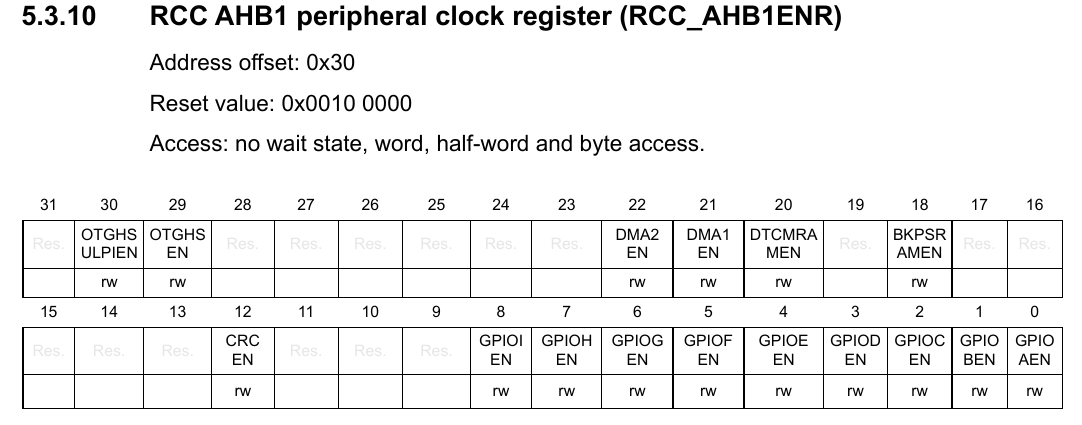
\includegraphics[width=\textwidth]{res/ahb1enr.png}
                \caption{Detalle de bits del registro \REG{AHB1ENR}}
                \label{fig:ahb1enr}
            \end{figure}

            Para estos casos, C nos permite una sintaxis como la siguiente, que nos deja acceder individualmente a nivel de bit a los registros:

            \begin{lstlisting}
                //Base address
                #define RCC_AHB1EN_BASE_ADDR 0x40023830

                //Structure for Reset and Clock Control peripheral clock register 1
                typedef union {
                    volatile uint32_t reg;

                    // 2. Access individual bits or bit-groups for the register above
                    struct {
                        volatile uint32_t GPIOAEN   	: 1;  // Bit 0: Enable peripheral (1 bit)
                        volatile uint32_t GPIOBEN   	: 1;  // Bit 1: Enable peripheral (1 bit)
                        ...
                    } bits;
                } RCC_AHB_ENR_TypeDef;

                //Handle:
                #define RCC_AHB1ENR 		((RCC_AHB_ENR_TypeDef *) RCC_AHB1EN_BASE_ADDR)
            \end{lstlisting}

            Posteriormente, podemos acceder a los campos individuales de la siguiente manera:

            \begin{lstlisting}
                RCC_AHB1ENR->bits.GPIOAEN = 1;
            \end{lstlisting}       

            Este registro en concreto es muy importante, pues activa los periféricos. De no activarlos, no funcionarán aunque se configuren adecuadamente.

    \subsection{Desarrollo de la práctica}
        
        Crea un BSP para que, en el código de la práctica anterior, no haya que acceder directamente a registros del periférico GPIOA. Necesitarás funciones para configurar \REG{MODER}, \REG{OTYPER}, \REG{OSPEEDR}, \REG{PUPDR} y también para escribir 1 o 0 (esto lo puedes hacer desde el registro \REG{ODR} o \REG{BSRR}). Consulta \REFMAN[6.4] para ver todos los registros y sus funcionalidades. Deberás:

        \begin{enumerate}
            \item Completar la definición de tipo para incluir todos los registros. También completar la definición de tipo de \REG{AHB1ENR}.
            \item Crear las funciones, junto con sus definiciones de valores, para controlar los diferentes registros.
            \item Empaquetar toda esta funcionalidad en un fichero \texttt{bsp.h} que irá dentro de la carpeta \texttt{Inc} del proyecto.
            \item Adaptar el código original \texttt{main.c} de la práctica para utilizar el BSP.
        \end{enumerate}
        

\end{document}